\chapter{LCD controller}
\section{LCD Controller}
Op de LCD zal de huidige tijd, ingestelde wekkertijd, datum en ingeschakelde functies te zien zijn. Een LCD is daar handig voor omdat het veel ontwerp vrijheid bied. Dat neemt ook mee dat het erg gecompliceerd kan worden. Het LCD dat zal worden gebruikt is van de fabrikant MIDAS, typenummer MC128064B6W-BNMLW. Het betreft een graphical LCD van 128 x 64 pixels met een register die geschreven kan worden. De bibliotheek met characters en de controller om het LCD te schrijven zal extern van deze chip plaatsvinden door middel van een atmega32-16pu. Deze keuze is gemaakt omdat voor de characters niet genoeg ruimte is op de chip. De LCD controller op de chip zal dus alleen de inkomende data moeten omzetten naar een positie waarnaar het geschreven moet worden en een bijbehorend character. De layout van het display is al vastgesteld, zodat de posities alvast bekend zijn.  Zie voor de layout afbeelding \ref{fig:lcdlayout}.  \\

\begin{figure}
  \centering
     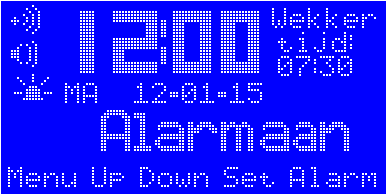
\includegraphics[angle = 0, scale= 1]{Figuren/LCD/voorbeeld_lcd.png}
       \caption{LCD layout}
\label{fig:lcdlayout}
\end{figure}

\section{Specificaties}

\begin{center}
\label{table:uitgangen}
\begin{tabular}{| l | l | p{4.5cm} |}
\hline
\textbf{Naam} & \textbf{Type} & \textbf{Functie} \\ \hline
clk           				& in std$\_$logic           									& Klok             \\ \hline
reset         			& in std$\_$logic           									& Reset            \\ \hline
ready					& in std$\_$logic 											&  \\ \hline
uren						&in std$\_$logic$\_$vector(5 downto 0) 		&data signaal met actuele uren afkomstig van DCF \\ \hline
minuten				&in std$\_$logic$\_$vector(6 downto 0) 		&data signaal met actuele minuten afkomstig van DCF \\ \hline
dagvdweek			&in std$\_$logic$\_$vector(2 downto 0)			&data signaal met de actuele dag afkomstig van DCF\\ \hline
dagvdmaand		&in std$\_$logic$\_$vector(5 downto 0) 		&data signaal met de actuele dag van de maand afkomstig van DCF \\ \hline
maand					&in std$\_$logic$\_$vector(4 downto 0) 		&data signaal met de actuele maand afkomstig van DCF  \\ \hline
jaar						&in std$\_$logic$\_$vector(7 downto 0)	 		&data signaal met het actuele jaar afkomstig van DCF  \\ \hline
dcf$\_$debug		&in std$\_$logic 												&signaal afkomstig van het dcf component en weergeeft of het DCF signaal ontvangen wordt of niet \\ \hline
menu					&in std$\_$logic$\_$vector(2 downto 0)			&data signaal die de actuele menu state weergeeft \\ \hline
alarm 					&in std$\_$logic												&buffer signaal dat weergeeft of alarmfunctie in of uitgeschakeld is\\ \hline
geluid$\_$signaal 		&in std$\_$logic 		 										&buffer signaal dat weergeeft of geluidsfunctie in of uitgeschakeld is \\ \hline
licht$\_$signaal 	&in std$\_$logic 		 										&buffer signaal dat weergeeft of lichtfunctie in of uitgeschakeld is  \\ \hline 
wektijd$\_$uren 	& in std$\_$logic$\_$vector(5 downto 0)		&data signaal met ingestelde wektijd uren \\ \hline 
wektijd$\_$min 	&in std$\_$logic$\_$vector(6 downto 0) 		&data signaal met ingestelde wektijd minuten \\ \hline 
data$\_$out 		&out std$\_$logic$\_$vector(6 downto 0) 		&data signaal dat de x,y,c informatie doorgeeft aan de microcontroller \\ \hline 
clk$\_$out 			&out std$\_$logic 		 										&clock om microcontroller clock mee te synchroniseren \\ \hline 
\end{tabular}
\end{center}

\newpage
\begin{figure}
  \centering
     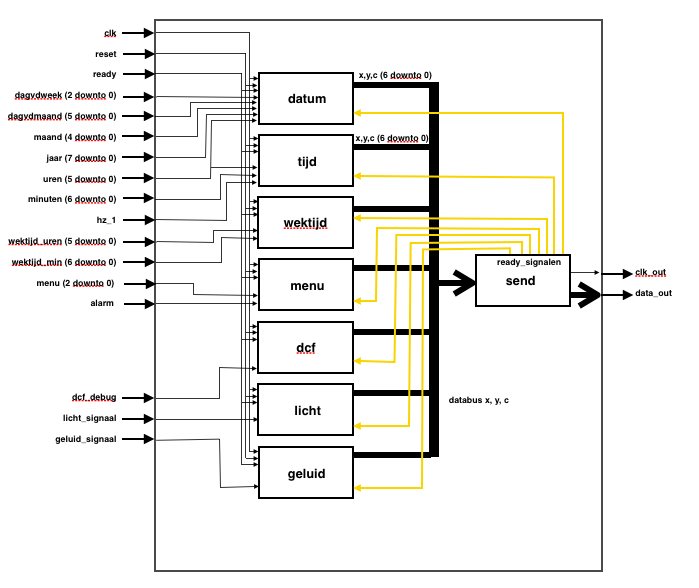
\includegraphics[angle = 0, scale= 0.75]{verslag_schemas/toplevel_entity.png}
       \caption{Toplevel Entity}
\label{fig:lcdtoplevel}
\end{figure}
\newpage

\subsection{Gedrag}
De LCD controller zal na de reset alle informatie die hij binnen krijgt omzetten naar een karakter met bij behorende x en y positie en wegschrijven naar de microprocessor van de LCD. Daarna zal de controller alleen de data die veranderd op de ingangen omzetten en  wegschrijven naar de microprocessor om tijd en onnodige acties te besparen. \\
Het verzenden van de x,y en c gaat door een data signaal van 7 bits samen met een clock$\_$out. Een neergaande klokflank geeft aan dat de data klaar staat om te verzenden zodat er op de opgaande klokflank kan worden gesampled. Zo zal eerst de x, daarna de y en als laatste de c worden verzonden. Het versturen van een karakter duurt dus 3 klokslagen van de clock$\_$out. een klokslag van de clock$\_$out is gelijk aan 2 klokslagen van de ingaande clk. 

\section{Functionaliteit}
De systemen links (datum, tijd, etc)  zorgen per stuk voor het ontvangen van de inkomende informatie en het omzetten naar een x,y positie met een karakter. De x,y en de c zal op de uitgang van het component worden gezet. 
Het component send$\_$buffer is een MUX en zorgt voor het uitlezen van de x,y en c en zal door middel van de ready signalen aangeven welk signaal hij heeft uigelezen en naar de zender heeft verstuurd. Zodra de ready laag wordt, weet het desbetreffende component dat de data is uitgelezen en zal daarna nieuwe data klaar zetten. 
Nadat de mux de data naar de zender heeft gebufferd, zal de zender de signalen een voor een door  verzenden naar de microcontroller. Tegelijkertijd zal de zender een clock$\_$out geven, zodra de clock laag wordt staat de data klaar, zodat op de opgaande klokflank de data vanaf de chip kan worden uitgelezen. 

\section{Subsystemen LCD}

\subsection{Datum}
\subsubsection{Gedrag}
Na een reset of \'e\'en keer per dag om 12 uur middernacht zal het datum component de data voor de nieuwe datum verzenden naar de zend buffer. De inkomende data is in het binary coded decimal (bcd) formaat. Eerst zal hij de dag van de week doorgeven, daarna de dag van de maand, de maand en daaropvolgend het jaartal. Dat allemaal sequentieel, getriggert op de neergaande klokflank van de ready$\_$buf. 

\begin{figure}
  \centering
     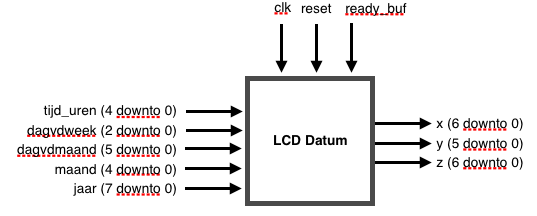
\includegraphics[angle = 0, scale= 0.75]{verslag_schemas/datum_entity.png}
       \caption{Entity datum}
\label{fig:datumentity}
\end{figure}


\subsubsection{Functionaliteit}
Het component werkt met een finite state machine (FSM) waarin de characters worden klaargezet en een counter genaamd positie wordt aangestuurd met daarnaast een apart process om de juiste input te bepalen afhankelijk van de counter. \\
Na de reset zal de FSM in de selectdata state starten en positie op 0 worden gezet. 
In het aparte process zal de de data$\_$buf worden gekoppeld aan de input die hoort bij positie=0 en zal de x en y bepaald worden. 
 In selectdata zal  afhankelijk van de counter (in dit geval 0) worden bepaald of de dag van de week of de getallen van de datum moet worden geschreven. Bij positie=0 zal het karakter van de dag van de week (in state cdvdw) worden klaargezet. Het karakter wordt bepaald door de waarde die op de data$\_$buf staat. Op de neergaande klokflank van het ready$\_$buf signaal zal de FSM terug gaan naar de state selectdata en zal er bij positie 1 worden opgeteld. Daardoor zal hierna het eerste getal van de datum worden geschreven. Dit zal zich herhalen tot positie =7, daarna zal hij naar de rust stand gaan en is de datum geschreven. \\
 Als het middernacht is, dus tijd$\_$uren = '00000', zal er ook een nieuwe datum worden klaargezet. Zodra de positie 7 is zal de machine in state selectdata blijven hangen totdat de tijd$\_$uren ongelijk is aan "00000". Dit om te voorkomen dat het component een uur lang onnodig data blijft verzenden. 


\subsubsection{FSM}
\begin{figure}
  \centering
     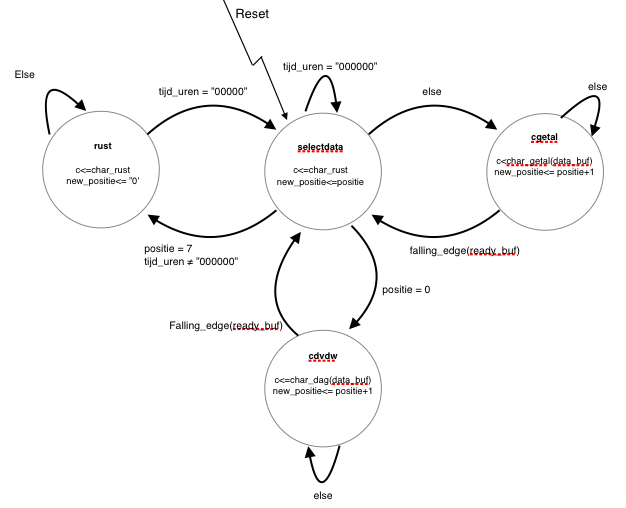
\includegraphics[width=15cm]{verslag_schemas/datum_fsm.png}
       \caption{FSM Datum}
\label{fig:lcddatumfsm}
\end{figure}

\subsubsection{VHDL code}
Zie \ref{code:ent_datum} voor de entity code. \\
Zie \ref{code:beh_datum} voor de behavioural code.\\
Zie \ref{code:tb_datum} voor de testbench die is gebruikt.
\subsubsection{Simulaties}
Zie \ref{fig:sim_datum_behavioural} voor de simulatie van de behavioural code. \\
Zie \ref{fig:sim_datum_circuit} voor de simulatie van het gesynthetiseerde circuit. 
De simulaties zijn uitgevoerd met een clock van 2000ns.  Er is getest tot 300k ns, zie de testbench in \ref{code:tb_datum} voor meer informatie.

\subsubsection{Resultaten}
Uit de simulaties is gebleken dat het circuit doet waarvoor het is ontworpen.

\subsection{Tijd en Wektijd}

\subsubsection{Gedrag}
Na een reset of bij het veranderen van de minuten zal de entity tijd data gaan verzenden. De data die verzonden wordt bevat informatie over welk character geprint moet worden en zijn positie. De characters die moeten worden verzonden worden bepaalt aan de hand van de minuten en uren die de entity in gaan. Dit zal altijd op de volgende volgorde gaan: tientallen uren, eentallen uren, tientallen minuten en als laatste eentallen minuten. Ook zal de module bij een opgaande flank van het \'e\'en Hz signaal de dubbele punt tussen de uren en minuten aan of uit zetten.\\
Het component wektijd verzend dezelfde informatie naar het LCD, alzij het op een andere positie. De wektijd zal beginnen met verzenden op het moment dat de wektijd wordt aangepast in het menu. De volgorde van de

\subsubsection{Functionaliteit}
Het component werkt volgens het Moore principe. Om de seconde wordt een nieuw character naar het LCD gestuurd. Dit character is voor de dubbele punt tussen de uren en minuten. Als er een minuut om is dan zal de nieuwe tijd naar het LCD worden verzonden.

\subsubsection{FSM}

\subsubsection{VHDL code}

\subsubsection{Simulaties}

\subsubsection{Testen}

\subsubsection{Resultaten}

\subsubsection{Discussie}

\subsection{Wektijd}

\subsubsection{Gedrag}

\subsubsection{Functionaliteit}

\subsubsection{FSM}

\subsubsection{VHDL code}

\subsubsection{Simulaties}

\subsubsection{Testen}

\subsubsection{Resultaten}

\subsubsection{Discussie}

\include{menu}
\include{dcf}
\include{geluidenlicht}

\subsection{VHDL code}
Zie \ref{code:ent_lcdtop} voor de entity code. \\
Zie \ref{code:beh_lcdtop} voor de behavioural code.\\
Zie \ref{code:lcdtop_tb} voor de testbench die is gebruikt.

\section{Simulatie}
Zie \ref{fig:sim_lcdtop} voor de simulatie van de behavioural code. \\
Zie \ref{fig:sim_lcdtop_circuit} voor de simulatie van het gesynthetiseerde circuit. \\

\section{Testen}
Tijdens het testen van verschillende subcircuits zijn veel dingen fout gegaan. Vaak waren de circuits dan ook wel goed, maar was de testbench niet correct. Zo hebben we in het begin met een te hoge clock frequentie getest, maar ook met signalen die niet lang genoeg hoog bleven. \\
Het systeem is ook getest op een Altera FPGA bord. Eerst dachten we dat het niet werkte, maar achteraf bleek dat, wat best logisch is,  het systeem zodanig snel werkt dat wij zelf het niet konden waarnemen. Door de klok te pulsen met een button konden we zien dat het systeem weldegelijk correct werkt.

\section{Resultaten}
De resultaten zijn goed. Het systeem heeft 2 errors in de switch level simulatie. Dat heeft te maken met de testbench waarin een situatie wordt gecre\"eerd die zich nooit zal voordoen. Dat maakt dus niks uit.

\subsection{Conclusie en discussie}
De controller werkt naar verwachting. Omdat vanwege tijdgebrek en gestelde prioriteiten de microcontroller nog niet af is voor het LCD kan nog niet worden getest of het systeem ook daarmee goed functioneerd. Al verwachten wij, omdat de simulaties en de test op de FPGA positief zijn, dat het kan gaan werken.\\
